\documentclass[10pt,a4paper]{article}
\usepackage[utf8]{inputenc}
\usepackage[turkish]{babel}
\usepackage[left=0.8in, right=1.0in, top=0.8in, bottom=.8in]{geometry}
\usepackage{amsmath}
\usepackage{amsfonts}
\usepackage{amssymb}
\usepackage{graphicx}
\usepackage{tikz}
\usepackage{fancyhdr}
\pagestyle{fancy}

\fancyhf{}
\fancyhead[L]{Robotes Robotik Çözümler}
\fancyhead[c]{Tren Dinamik Modeli}
\rhead{ \fancyplain{}{\today} }
\rfoot{ \fancyplain{}{\thepage} }


\author{Robotes Robotik Çözümler}
\title{Tren Dinamik Model Raporu }

\begin{document}

\maketitle
\newpage

\tableofcontents
\newpage

\section{Giriş}
Bu rapor da Robotes Robotik Çözümler tarafından geliştirilen tren simülatör dinamik model yazılımı incelenmektedir. Geliştirilecek olan sistemin hareket denklemleri, modelleri, yazılım geliştirme süreci anlatılmaktadır. Bu belge henüz bitmemiştir, proje ilerlemesiyle beraber ilerleyecektir. Rapor versiyonu 0.1. 
 
\subsection{Amaç}
Raporda anlatılan yazılım Savronik A.Ş. tarafından geliştirilen tren simülatörü projesi için geliştirilmektedir. Amaç Savronik tarafından geliştirilen görsel arayüz, ve tren kokpit model sistemininin  kullanacağı bir dinamik model geliştirmektir. Yazılım gerçek zamanda çalışan ve tren dinamik sistemini hesaplayan bir dinamik model motorudur. 

\subsection{Robotes Robotik Çözümler}
Robotes Robotik Çözümler her türlü mekanik, elektronik ve yazılım sistemlerinin birleşimi üzerinde 
çalışan bir firmadır. ESOGÜ Teknoparkta bulunan ofisiyle AR-GE projeleri yapmaktadır. İletişim için robotes@robotes.com.tr.


\subsection{Rapor İçeriği}
Öncelikle oluşturulan matematik modeli anlatılacaktır. Bu model gerçek trenin çalışma şeklini taklit etmeye çalışmaktadır. Bunu yaparken bazı varsayımlar yapılmıştır. Bu varsayımlarla birlikte sistemi en iyi şekilde modellemek çalışılmıştır. Özel olarak verilen değerler 43000 Lokomotif modeli için geçerlidir.

Daha sonra oluşturulan matematik modelin yazılıma geçirilmesi incelenmiştir. Oluşturlan her sınıf incelenmiş ve UML diyagramı verilmiştir. Sistemin kurulumu ve oluşturulan doxygen bilgisi eklenmiştir.

Sistem hazırlandıktan sonra performans ve doğruluk ölçcen testlerden bahsedilmiştir. Bu testler sayesinde sistemin doğru çalıştığı gösterilmeye çalışılmıştır. 

En son kısımda sisteme eklenmesi planlanan şeyler anlatılmıştır. Bu kısımlar zaman ilerledikçe sisteme eklenecektir.

  
\newpage

\section{Matematik Modeli}

Bu bölümde sistemin matematik modeli oluşturulacaktır. Bu model gerçeğe mümkün olduğunca yakın olmalı fakat hesapları gerçek zamanlı yapabilmek için basit olmalıdır. Öncelikle genel hareket denklemi gösterilmiş sonra da hesaplar detaylı şekilde incelenmiştir.


\subsection{Genel Hareket Denklemi}
Genel hareket denklemi (\ref{hareket_denklemi}) hesaplanan kuvvetlere göre lokomotif ve vagonların ivmelerini hesaplar.  Bu denklem seti, denklem çözücü tarafından çözülecek ve ivme değerlerinden hız ve pozisyon değerleri hesaplanacaktır.

\begin{equation}
\label{hareket_denklemi}
F_{i-1}^{i}+F_r^i  + F_{i+1}^i = m^i\ddot{x}^i
\end{equation}
$\newline
F_r: \text{etkiyen kuvvet (kayıp kuvvetler, fren, motor\ldots)} \\
F_i^{i+1}: \text{i. araçtan i+1. araca olan kuvvet} \\
i: \text{index numarası} \\
m: \text{kütle} \\
\ddot{x}: \text{ivme} \\
\dot{x}: \text{hız}\\
x: \text{pozisyon}\\
$
Hareket denklemi 3 adet bilinmeyen içermektedir: $F_(i-1)^i$, $F_i^(i+1)$, $\ddot{x}$. Araçlar arası kuvvetler direk olarak araçlar arasındaki uzaklığa bağlı olduğu için hesaplanabilirler. Böylece iki bilinmeye bulunarak tek bilinmeyen kalır. Hareket denklemi düzenlenerek aşağıdaki denklem (\ref{ivme_denklemi}) bulunur.

\begin{equation}
\label{ivme_denklemi}
\ddot{x}^i=\dfrac{F_{i-1}^{i}+F_r^i+F_{i+1}^{i}}{m^i}
\end{equation}
Bu denklem kullanılarak hız ve pozisyon şu şekilde hesaplanır.

\begin{eqnarray}
\dot{x}^i(t)=\dot{x}^i(t-1)+\ddot{x}^i(t)*\Delta t \\
x^i(t)=x^i(t-1)+\dot{x}^i(t)*\Delta t
\end{eqnarray}


\subsection{Araçlar Arası Kuvvetler}
Araçlar arasındaki kuvvetler araçlar arasındaki uzaklığa bağlıdır. Bu ilişki uzaklık artarken ve azalırken farklı karakteristikler göstermektedir. Bu ilişki en iyi şekil~\ref{image:kanca_kuvvetleri} ile anlatılabilir. Burada Türkiye’de kullanılan tren modellerine uygun katsayıları kullanılmalıdır. Bu katsayılar tecrübe edilmiş kuvvetlere göre hesaplanmıştır.

Şekil~\ref{image:kanca_kuvvetleri} deki temel mantık şöyledir. Ortada kuvvet olmayan kısım vagonlar arasındaki boşluğu ifade etmektedir. Bu boşluk esnasında kuvvet oluşmaz. Kırmızı ile gösterilen kısımlarda uzaklık artarken büyüklük olarak çok olan kuvvet oluşur yani sağ tarafta artarken üstteki sol tarafta azalırken alttaki kuvvet görülür. Uzaklık değerı sıfıra yaklaşırken ise düşük olan kuvvet oluşmaktadır. 

\begin{figure}[h]
\shorthandoff{=}
\centering
\caption{Araçlar Arası Kuvvet}
\label{image:kanca_kuvvetleri}
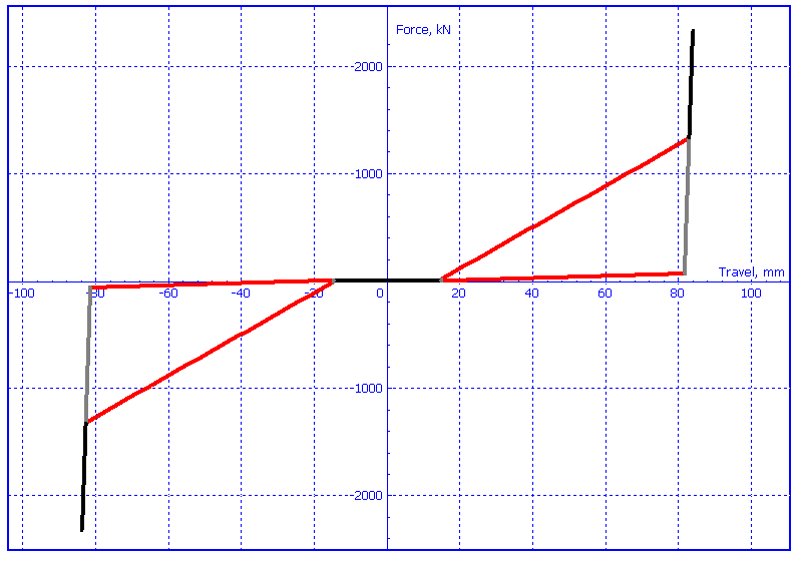
\includegraphics[scale=0.7]{resimler/kanca_kuvvetleri.png} 
\end{figure}

\newpage


\subsection{Fren Sistemi}
Fren sistemi 3 ana başlık içinde incelenmiştir. Öncelikle fren sinyalini taşıyan kondüvit hattı anlatılmıştır. Kondüvit hattındaki basınca göre fren sistemini kontrol eden kontrol valfı anlatılmış ve daha sonra basınç fren ilişkisi verilmiştir. Şekil~\ref{image:fren_sistemi} de fren sisteminin basit bir gösterimi verilmiştir. Kondüvit hattı basınç ile makinist tarafından verilen fren komutunu vagonlara iletir. Kondüvit hattındaki basınca göre farklı tepkiler veren kontrol valfı yedek hava deposundaki havayı kullanarak fren silindirini doldurur böylece fren yapılmış olur. 

\shorthandoff{=}
\begin{figure}[!h]
\centering
\caption{Basit Fren Sistemi}
\begin{tikzpicture}
\filldraw[fill=red,draw=black] (0,0) .. controls (0,0.555) and (-0.455,1) .. ++(-1,1) -- node[below=0.2cm] {43000} ++(-2,0) -- ++(0,-1) --cycle ;

\draw[thin,gray] (0,-0.2) -- (-17,-0.2) ;
\foreach \x in {-4,-8,-12}
\filldraw[fill=blue,draw=black] (\x,0) -- ++ (0,1) -- ++(-3,0) -- ++(0,-1) --cycle;

\filldraw[fill=blue,draw=black] (-16,0) -- ++ (0,1) -- ++(-1,0) -- ++(0,-1) --cycle;

\filldraw[thick,double] (-2,0.2) -- (-3.3,0.2);
\foreach \x in {-3.7,-7.7,-11.7}
\draw[thick,double] (\x,0.2) -- ++(-3.6,0);
\foreach \x in {-3.3,-7.3,-11.3,-15.3}
\draw[thick,double] (\x,0.2) arc [start angle=0, end angle=-180, radius = 0.2];

\draw[thick,double] (-15.7,0.2) -- ++(-1.3,0);

\foreach \x in {-0.5,-4.5,-8.5,-12.5}
\filldraw (\x,-0.1) circle [radius=0.1] ++(-2,0) circle [radius=0.1];
\filldraw (-16.5,-0.1) circle [radius=0.1];

\draw[->] (-11.7,0.2) .. controls ++(0,0.555) and ++(0,0) .. (-12,1.5) node[above=0.1cm] {Konduvit Hattı $P_{bp}$};

\draw[red] (-13,0.2) circle [radius=0.1] -- (-13,-2);

\draw[thick,double] (-10,-2) -- ++ (-5,0) node[above=0.1cm] {Kondüvit Hattı};
\draw[thick,double] (-12,-2) -- ++ (0,-1)  circle [radius=1,below=1cm] node [below=2cm]{Kontrol Valfı};
\draw[thick,double] (-13,-4) -- ++ (-1,0);
\draw[thick,double] (-11,-4) -- ++ (1,0);
\draw[thick,double,blue] (-14,-3) node [below=1cm,left]{Yedek Hava Deposu} rectangle ++(-3.5,-2);
\draw[thick,double,blue] (-6.5,-3) node [below=1cm,left=0.5cm]{Fren Silindiri} rectangle ++(-3.5,-2);
\draw[thick] (-6.5,-4) -- ++ (1,0) -- ++ (-1,-2) circle(0.1) -- ++ (-0.5,-1) ++(-0.25,-1) arc (-30:30:2) node[below=2cm]{Fren Pabucu} ;
\draw[thick] (-8.3,-7) circle(1) node {Tekerlek};
\end{tikzpicture}
\label{image:fren_sistemi}
\end{figure}


\subsubsection{Kondüvit Hattı Basınç Dağılımı}
Kondüvit hattı içindeki basınç $P_{bp}$ lokomotifte bulunan makinist musluğu tarafından kontrol edilir. Bu basınç sayesinde fren sinyali vagonlara aktarılır. Kondüvit hattında basınç olduğu zaman fren yapılmaz ve basınç azaldığı zaman basınç değerinin azalma miktarına orantılı olarak fren yapılır. Bu bölümde makinist musluğu ile kondüvit basıncı arasındaki ilişki incelenecektir.\\

Şekil~\ref{image:makinis_musluk} de makinist musluğunun olduğu konumlar verilmiştir. Bu konumlara göre oluşan tepkiler Tablo~\ref{table:makinist_musluk} da verilmiştir.


\shorthandoff{=}
\begin{figure}
\centering
\caption{Makinis Musluğu Konumuna göre Etkileri}

\begin{tikzpicture}[scale=2]
\shorthandoff{=}
\draw (1,0) arc [start angle=0, end angle= 180, radius = 1];
\foreach \angle in {30,60,90,120,150}
	\draw[dashed,red] (0,0) -- (\angle:1); 
\foreach \angle in {30,60,90,120,150}
	\draw[thick,double,red] (\angle:1) -- (\angle:2);

\filldraw[fill=blue!50!gray,draw=blue] (30:2) circle [radius=0.1] node[text width = 4cm,below=0.8cm,right=0.5,black]{Seri Fren ve \\ Totmandan Kurtarma};

\filldraw[fill=blue!50!gray,draw=blue] (60:2) circle [radius=0.1] node[right=0.4cm,black]{Kademeli Fren};

\filldraw[fill=blue!50!gray,draw=blue] (90:2) circle [radius=0.1] node[above=0.4cm,black]{Yol Durumu};

\filldraw[fill=blue!50!gray,draw=blue] (120:2) circle [radius=0.1] node[text width = 2cm,left=0.5,black]{Kademeli Tahliye};

\filldraw[fill=blue!50!gray,draw=blue] (150:2) circle [radius=0.1] node[text width = 3cm,below=0.8cm,black]{Seri Doldurma ve \\ Tahliye};
\end{tikzpicture}
\label{image:makinis_musluk}
\end{figure}


\begin{table}[!h]
\centering
\caption{Makinist Musluğu Tepkileri}
\begin{tabular}{|c|c|c|}
\hline 
Konum Değeri & Konum İsmi & Tepki \\ 
\hline 
0 & Seri Doldurma & Kondüvit hattını 7KPa doldur \\ 
\hline 
1 & Kademeli Tahliye & Kondüvit Hattını doldur \\ 
\hline 
2 & Yol Durumu & Tepki Yok \\ 
\hline 
3 & Kademeli Fren & Boşalt \\ 
\hline 
4 & Seri Fren & Tümüyle Boşalt (0KPa)\\ 
\hline 
\end{tabular} 
\label{table:makinist_musluk}
\end{table}

\subsubsection{Modrabl}

\subsubsection{Purjör}


\paragraph{Seri Doldurma}
Seri doldurma, freni hızlı şekilde açmak için kondüvit basıncını normal basıncın (5KPa) üstüne 7kPa a çıkartır. 7KPa konumunda 15 saniye boyunca tutulur ve daha sonrasında 5 saniyede 5.4Kpa a düşürülür. Sonradan 5.4 KPa dan 5.0 Kpa a düşürme süresi 220 saniyedir. Böylece frenle hızlı bir şekilde çözülmüş olur.
\paragraph{Kademeli Tahliye}
Kademeli tahliye makinistin kondüvit sisteminin basıncını arttırması için kullanılır. Basınç kademeli olarak artarak fren miktarını azaltma sağlaır. Sistem adımda 0.2 kPa arttırır. Gerçek zamanlı bir sistemi için buna yaklaşık olarak saniyede 0.05 kPa azaltılarak sağlanır.
\paragraph{Yol Durumu}
Yol durumunda kondüvit borusundaki basınç değişmez. Makinist kolu bıraktığında kol bu duruma döner ve sisteme bir etki yapılmaz.
\paragraph{Kademeli Fren}
Kademeli fren makinistin kondüvit sisteminin basıncını azaltması için kullanılır. Basınç kademeli olarak azalarak fren miktarında arttırma sağlanır. Sistem adımda 0.2 kPa azaltır. Gerçek zamanlı bir sistemi için buna yaklaşık olarak saniyede 0.05 kPa azaltılarak sağlanır.
\paragraph{Seri Fren}
Seri fren trenin hızlı şekilde fren yapması için kullanılır. Kondüvit basıncı acil bir şekilde 5 sn de ??? 0 kPa a düşürülür ve sistemin fren yapması sağlanır.

\newpage

\subsubsection{Kontrol Valfı}
Kontrol valfı kondüvit hattındaki basınç değişimine göre fren silindirindeki basıncı değiştirir, fren silindirindeki basıncı değiştirmek için yedek hava deposunu kullanır. Fren silindirinde basınç yokken fren olmaz, fren silindirine hava doldukça fren pabucu hareket eder ve tekerleğe baskı yaparak fren yapılır. Kontrol valfının farklı basınçlarda davranış şekli Tablo da verilmiştir.


\subsubsection{Basınç Fren İlişkisi}
Fren silindirinde oluşan basınç sonucu fren pabucu tekerleğe baskı uygulamaktadır. Bu basınç değerıne bağlı olarak bir sürtünme kuvveti oluşmaktadır. Burada fren silindirindeki basınç $P_{bc}$ ile fren kuvveti arasındaki ilişki anlatılmaktadır.

Fren silindirinde oluşan basınç öncelikle silindir içindeki yayı ittirmektedir. Silindir maximum strok konumuna geldiğinde basınç değeri tekerleğe aktarılmaktadır yani basıncın oluşturduğu kuvvet yay kuvvetine eşit ve büyük olduğunda fren kuvveti aktarılmaktadır. 

\begin{equation}
P_{bc} \times A_{bc} = F_{bc}
\end{equation}  
$\newline
P_{bc} : \text{Fren silindiri basınç değeri (kPa)}\\
A_{bc} : \text{Fren silindiri kesit alanı }(m^2) \\
F_{bc} : \text{Fren silindiri içinde basınç tarafından yapılan kuvvet (N)}
$

Fren silindiri üzerindeki kuvvet bir kol aracılığıyla pabuçlara aktarılır ve sürtünme kuvvetine dönüşür. Tekerlek üzerine etki eden kuvvet pabuç sayısıyla çarpılarak araca etki eden kuvvet bulunur.

\begin{equation}
F_{d} = (F_{bc} - k_{bc} \times x_{bc}) \times \epsilon_{bc} \times l_b \times \epsilon_l \times \mu_b \times n_b  
\end{equation}
$\newline
F_d : \text{Bir tekerlek üzerindeki sürtünme kuvveti değeri}\\
k_{bc} : \text{Yay katsayısı}\\
x_{bc} : \text{Fren silindirinin hareket miktarı, yayın sıkışma miktarı}\\
\epsilon_{bc} : \text{Fren silindirinin verimi}\\
l_b : \text{Kuvvet aktarma kolu oranı}\\
\epsilon_l : \text{Kuvvet aktarma kolu verimi}\\
\mu_b : \text{Sürtünme katsayısı}\\
n_b : \text{Fren pabucu sayısı}\\
$


\subsection{Sürtünme ve kayıp kuvvetler}
Tren üzerine farklı nedenlerden dolayı enerji kaybettiden kuvvetler etki etmektedirler. İki tür enerji kaybettiren kuvvet vardır; kurb direnci ve seyir direnci. İlave olarak trene rampa direnci etki eder, fakat bu kuvvet eğime göre enerji artırır veya azaltır.

\begin{align}
F_{seyir} &= \text{N cinsinden seyir direnci}  \nonumber \\
F_{kurb} &= \text{N cinsinden kurb direnci}  \nonumber \\
\dot{x}_{km} &= \dfrac{km}{h} \text{ cinsinden hız}  \nonumber \\
n_a &= \text{teker eksenı sayısı} \nonumber \\
m_t &= \text{ton cinsinden kütle} \nonumber \\
r_c &= \text{kurb yarıçapı} \nonumber \\
F_{rampa} &= \text{Rampa direnci} \nonumber \\
s &= \text{yolun eğimi} \nonumber \\
\end{align}

\subsubsection{Seyir Direnci}
Seyir direnci araç çeşidine göre değişmektedir. Bu değişim araçların yapılarından ve konumlarından kaynaklanmaktadır.
\begin{itemize}
\item \textbf{Lokomotif Seyir Direnci}
\begin{equation}
F_{seyir} = (6.5 \times m_t) + (130 \times n_a) + (0.1 \times m_t \times \dot{x}_km) + (0.3 \times \dot{x}^2_{km})
\end{equation}

\item \textbf{Yük Vagonu Seyir Direnci}
\begin{equation}
F_{seyir} = (2 + \dfrac{0.057 \times \dot{x}^2_{km} }{100})\times m_t \times 10
\end{equation}

\item \textbf{Yolcu Vagonu Seyir Direnci}
\begin{equation}
F_{seyir} = (1.986 + 0.00932 \times \dot{x}_km + 0.000161 \dot{x}^2_{km}) \times m_t
\end{equation}
\end{itemize}

\subsubsection{Kurb Direnci}
Kurb direnci kurblarda tren üzerine etki eden bir kuvvettir. Bu kuvvet kurbun yarıçap uzunluğuna bağlıdır.

\begin{equation}
F_{kurb} = \dfrac{6500}{r_c - 55} \times m_t
\end{equation}

\subsubsection{Rampa Direnci}
Rampa dinrenci yolda olan eğim sonucu yerçekimi kuvvetinin trene etkimesidir. Bu kuvvet eğim eksi ise pozitif, eğim pozitif ise negatf etki yapar.

\begin{equation}
F_{rampa} = s \times m_t
\end{equation}

\subsection{Aderans (Patinaj ve Kayma)}
Patinaj yol ile tekerlek arasında yeterince sürtünme kuvveti olmadığı zaman oluşur ve bu modelde motor ve fren kuvvetlerinin etkisini tümüyle yok eder. Öncelikle patinaj durumunun oluşup oluşmadığı bulunmalıdır, bunun için aderans katsayısı hesaplanır ve oradan da aderans kuvveti hesaplanır. Tekerleğe etki eden kuvvet bu aderans kuvvetinden büyükse kayma gerçekleşir. 

\begin{align}
\mu &= \text{tekerlek ve ray arasındaki sürtünme katsayısı} \nonumber \\
\mu_a &= \text{aderans katsayısı} \nonumber \\
F_{aderans} &= \text{aderans kuvveti} \nonumber \\ 
\end{align}

\begin{equation}
\mu_a = \mu \dfrac{8+0.1 \times \dot{x}_{km}}{8+0.2 \times \dot{x}_{km}}
\end{equation}

\begin{equation}
F_{aderans} = m_t\times \mu_a
\end{equation}

Maksimum kuvvet bu şekilde hesaplanır. İleride tekerlek başına düşen motor ve fren kuvvetleri hesaplanırken bu değer ile karşılaştırılacaktır.

\subsection{Motor ve Dinamik Fren}
Lokomotif için motor ve dinamik fren verileri üretici tarafından sağlanmaktadır. Bu projede modellenen 43000 lokomotifi için de bu değerler bir grafik olarak verilmiştir. Bu grafikten gereken verilerin elde edilmesi için eğrilere karşılık gelen polinomlar bulunmuştur. Bu bulunan polinomlar aşağıda grafikleri ile birlikte verilmiştir.

\subsubsection{Motor Bilgileri}
Şekil~\ref{image:motor_kuvveti} bir teker eşındeki motor kuvveti göstermektedir, yani bir lokomotifte 6 tane teker eşi var ise toplam kuvvet bu grapfikteki kuvvetin 6 katıdır.

\begin{figure}[!h]
\shorthandoff{=}
\centering
\caption{Teker Eşi üzerindeki Motor Kuvvet}
\label{image:motor_kuvveti}
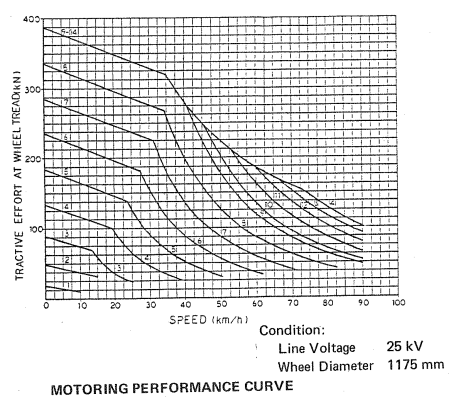
\includegraphics[scale=0.7]{resimler/motor.png} 
\end{figure}

Denklemleri aşağıda listelenmiştir (düzeltilecek):
\begin{align}
&1) \hspace{5mm} F = 0.9050 \times V + 5.471 \hspace{5mm} [5,90] \\
&2) \hspace{5mm} F = 1.203 \times V + 4.986 \hspace{5mm} [5,79] \nonumber \\
&3) \hspace{5mm} F = 1.571 \times V + 8.143 \hspace{5mm} [5,68] \nonumber \\
&4) \hspace{5mm} F = 1.982 \times V + 9.089 \hspace{5mm} [5,61] \nonumber \\
&5) \hspace{5mm} F = 2.51 \times V + 9.449 \hspace{5mm} [5,54] \nonumber \\
&6) \hspace{5mm} F = 3 \times V + 13 \hspace{5mm} [5,49] \nonumber \\
&7) \hspace{5mm} F = 3.6 \times V + 15 \hspace{5mm} [5,45] \nonumber \\
&8) \hspace{5mm} F = 4.338 \times V + 14.31 \hspace{5mm} [5,37.5] \nonumber \\
&9) \hspace{5mm} F = 5.074 \times V + 14.63 \hspace{5mm} [5,32] \nonumber \\
&10) \hspace{5mm} F = 5.609 \times V + 19.96 \hspace{5mm} [5,28] \nonumber 
&7) \hspace{5mm} F = 3.6 \times V + 15 \hspace{5mm} [5,45] \nonumber \\
&8) \hspace{5mm} F = 4.338 \times V + 14.31 \hspace{5mm} [5,37.5] \nonumber \\
&9) \hspace{5mm} F = 5.074 \times V + 14.63 \hspace{5mm} [5,32] \nonumber \\
&10) \hspace{5mm} F = 5.609 \times V + 19.96 \hspace{5mm} [5,28] \nonumber 
\end{align}
\subsubsection{Dinamik Fren Bilgileri}
Şekil~\ref{image:dinamik_fren} bir teker eşindeki dinamik fren kuvvetini göstermektedir, yani bir lokomotifte 6 tane teker eşi var ise toplam kuvvet bu grapfikteki kuvvetin 6 katıdır.

\begin{figure}[!h]
\shorthandoff{=}
\centering
\caption{Teker eşi üzerindeki Dinamik Fren }
\label{image:dinamik_fren}
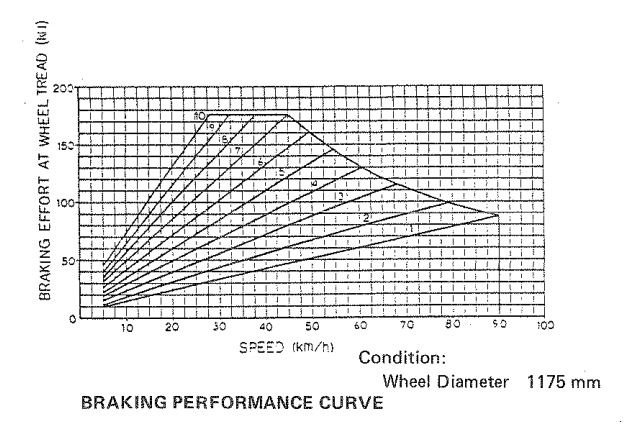
\includegraphics[scale=0.7]{resimler/dinamik_fren.jpg} 
\end{figure}

10 kademenin modeli denklem seti~\ref{dinamik_fren_model} de verilmiştir, her denklemin yanında tanımlı olduğu hız aralığı verilmiştir:

\begin{flalign}
\label{dinamik_fren_model}
&1) \hspace{5mm} F = 0.9050 \times V + 5.471 \hspace{5mm} [5,90] \\
&2) \hspace{5mm} F = 1.203 \times V + 4.986 \hspace{5mm} [5,79] \nonumber \\
&3) \hspace{5mm} F = 1.571 \times V + 8.143 \hspace{5mm} [5,68] \nonumber \\
&4) \hspace{5mm} F = 1.982 \times V + 9.089 \hspace{5mm} [5,61] \nonumber \\
&5) \hspace{5mm} F = 2.51 \times V + 9.449 \hspace{5mm} [5,54] \nonumber \\
&6) \hspace{5mm} F = 3 \times V + 13 \hspace{5mm} [5,49] \nonumber \\
&7) \hspace{5mm} F = 3.6 \times V + 15 \hspace{5mm} [5,45] \nonumber \\
&8) \hspace{5mm} F = 4.338 \times V + 14.31 \hspace{5mm} [5,37.5] \nonumber \\
&9) \hspace{5mm} F = 5.074 \times V + 14.63 \hspace{5mm} [5,32] \nonumber \\
&10) \hspace{5mm} F = 5.609 \times V + 19.96 \hspace{5mm} [5,28] \nonumber 
\end{flalign}

Üst eğri iki parçaya ayrılmıştır. Denklem~\ref{dinamik_fren_lineer} lineer olan kısmı, denklem~\ref{dinamik_fren_parabolik} parabolik olan kısmı modellemektedir.
\begin{equation}
\label{dinamik_fren_lineer}
F = 0 \times V + 177 \hspace{5mm} [28,45] \\
\end{equation}

\begin{equation}
\label{dinamik_fren_parabolik}
F =  \dfrac{-0.6589\times V^2 + 130.6 \times V - 537.9}{V - 22.36} \hspace{5mm} [45,90] \\
\end{equation}

\newpage

\subsection{Kabuller ve Varsayımlar}
Matematik modeli oluşturulurken belli varsayımlar ve kabuller yapılmıştır. Bu kabuller modelin hassasiyetini ve doğruluğunu belirleyecektir. Önemli olan bu kabullerin iyice incelenip oluşacak hatalar ile olan bağlantılarını bulabilmektir.

\newpage
\section{Yazılım Modeli}
Güncellenmesi gerekiyor.
\subsection{XML Parser (C++) Kütüphanesi Seçimi, Kullanım Şekli ve Optimal Tasarım}
Geliştirilecek olan uygulamada kullanılacak verilerin tutulması ve yaratılacak nesnelerin (yol, lokomotif ve vagon) karakteristik özelliklerinin kullanıcı tarafından girilmesi gerekmektedir. Bu işlem dinamik akış esnasında bir dosya üzerinden okunması ve kullanıcının da söz konusu dosyaya gerekli bilgileri, gerekli yapıda girmesi gerekmektedir. Bu işlemlerin gerçekleştirilmesinde kullanılacak dosya tipi “XML” olarak belirlenmiştir. XML, hızlı veri işleme ve bu işlemi gerçekleştirmek için yaratılmış harici kütüphaneleri ile uygun bir  dosya tipidir. 
XML dosyalarının işlenmesinde kullanılabilecek pek çok kütüphane mevcuttur. TinyXml ve PugiXml mevcut kütüphanelerin en popüler olanlarıdır. Söz konusu kütüphaneler mevcut hız karakteristiği, kullanım kolaylığı ve mevcut yazılıma entegrasyon uygunluğu ile göz doldurmaktadır.
Oluşturulacak yazılımda PugiXml,  hız karakteristiği, kullanım kolaylığı ve yazılım entegrasyonunun uygunluğundan dolayı tercih edilmiştir.
Geliştirilecek olan uygulamada, önceden yaratılmış XML dosyalarının okunması ve okunan dosyalara bağımlı nesnelerin yaratılması işlemini üstlenecek sınıfların tasarlanması hedeflenmiştir. Tasarlanan sınıflar yol bilgisini içeren XML dosyalarını okuyup, okunan XML dosyasının içerdiği bilgiyi, ilintili olduğu sınıf tipinde nesneye aktaracaktır.
Elde edilen yapı, mevcut tasarım içerisinde yaratılış ve dosya okuma işlemlerini üstlenmekte ve kullanıcının yaratılış aşamasında yapması gereken işlemleri minimum seviyeye indirmektedir.

\begin{figure}[h]
\shorthandoff{=}
\centering
\caption{Parser Modeli}
\label{image:parser}
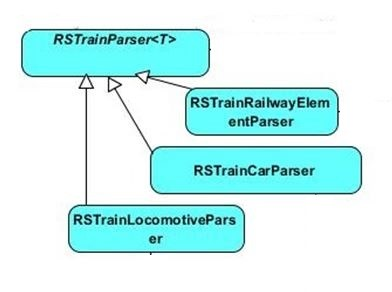
\includegraphics[scale=0.8]{resimler/parser.jpg} 
\end{figure}

\subsection{Diferansiyel Denklem Çözücü (C++) Kütüphane Seçimi, Kullanım Şekli ve Optimal Tasarım}
Geliştirilecek olan tren dinamik model tasarımının matematiksel modeli diferansiyel denklemler içermektedir. Söz konusu diferansiyel denklemler, tren modelinin dinamik hareketini modellemekte ve sistemin akışı esnasında sürekli çözüme ihtiyaç duymaktadır. 
C++ ortamında diferansiyel denklem çözümü ve İntegrasyon işlemini gerçekleştirebilmek için kullanılabilecek kütüphanelerin başında “boost-odeint” kütüphanesi gelmektedir.  Boost-odeint kütüphanesi oluşturulan diferansiyel denklem modelini kullanıcının tanımladığı aralıklarda çözümleme yeteneğine sahiptir. İntegrasyon işlemini numerik metotları kullanarak gerçekleştirmektedir ve kullanıcı konfigürasyonuna açıktır.
Mevcut sistemde kullanılacak olan boost-odeint kütüphanesinin sahip olduğu integrasyon metotlarından dördüncü derece runga-kutta kullanılması hedeflenmiştir. Bu metot integrasyon step aralığının kullanıcı tarafından değiştirilmesine izin vermesi , adım integrasyonu yaklaşımının gerçekleştirilebilmesi ile ön plana çıkmaktadır.
Tren  modelin çözümlenebilmesi için, sistemin diferansiyel modelinin sistemde tutulması ve integrator tarafından bu modelin bilinmesi gerekmektedir. Söz konusu modelin tanımlanması, kullanıcı tarafından yaratılan bir veri tipi (struct ya da class) ve bu veri tipinin sahip olduğu parantez operatörü fonksiyonu üzerinden gerçekleştirilmektedir. İntegrator bu modeli kullanarak kullanıcı tarafından verilen aralıkta sistem çözümünü gerçekleştirmektedir. Tasarlanan sistem modelinde ihtiyaç duyulan çıktılar sistemin pozisyonu, hızı ve ivmesidir. Mevcut diferansiyel modelde bu çıktıları üretecek şekilde tasarlanmıştır.  

\subsection{Thread Temelli Yapı ve Kontrolü}
Geliştirilen simulator sisteminin dinamik ve dinamik modele bağımlı matematiksel modelinin gerçek zamanlı çözümlemesi beklenmektedir. Fakat gerçek  zamanlı çözüm işlemini başlatan fonksiyonun çağrılması sistemi istemli şekilde oluşturulmuş sonsuz döngüye sokmaktadır. Bu işlem sistemi kullanıcı kontrolü dışına çıkarmakta ve tepkisiz hale getirmektedir. Bu durumun önüne geçmek için matematiksel modelin çözümlenmesini farklı bir  “Thread” e devretmek gerekmektedir. 
C++ ortamında geliştirilmiş bağımsız Thread kütüphaneleri bulunmaktadır. Bu kütüphanelerin içerisinde genel kabullenme görmüş en yaygın kütüphane Boost-Thread kütüphanesidir. Boost-Thread kütüphanesi yardımı ile sistemde ortaya çıkan tepkisiz kalma sorunu aşılmaktadır.

\subsection{Grafik Çizimi için Üst Seviye Dil Seçimi}
C++ ortamında geliştirilmiş tren dinamik model kütüphanesi tarafından elde edilen sonuçların, kod akışı esnasında görüntülenmesi ve hareket halindeki tren sisteminin dinamik kontrolünün sağlanması, geliştirme sürecinde testlerin yapılabilmesi için, üst seviye kontrol diline ihtiyaç duyulmaktadır. Bu dil hızlı bir şekilde kullanıcı ara yüzü hazırlamaya uygun olmalı ve gerçek zamanlı grafik çizim kütüphanelerine sahip olmalıdır. Bu şartları sağlayan üst seviye dillerin başında Python ve Java gelmektedir. 
Kullanım kolaylığı optimize edilmiş grafik  açık kaynaklı grafik kütüphanesi ile Java tercih edilip, JFreeChart kütüphanesi kullanılmıştır. !!!!!! resim eklenecek

\subsection{C++ ve Üst Düzey Dilin Birleştirilmesi}
C++ dilinde yazılan tren dinamik model uygulamasının üst seviye diller yardımıyla görsel arayüz ve grafik ortamında test edilebilmesi için kaynak kodlarının hedef üst seviye dil için dll olarak derlenmesi gerekmektedir. Bu işlemi optimal olarak gerçekleştirebilmek kullanılacak araçlardan biri SWIG dir. 
SWIG, C++ yada C dilinde yazılmış kaynak kodlarının üst seviye dillerde kullanılabilmesini sağlayan araçtır. Bu araç hedef  üst seviye dil için C++ yada C de yazılmış kaynak kodlarının eşdeğer C karşılıklarını barındıran adaptör kaynak kütüphanesi yaratır. Geliştirici tarafından yazılan esas kaynak kodlarının yanında SWIG tarafından yaratılan adaptör kaynak kütüphanesi de derlenir ve elde edilen dll dosyası hedef üst seviye dile dahil edilip kullanılır.

\subsection{UML Tasarımı}
Geliştirilecek yazılımın tasarım aşaması Visual Paradigm UML Designer aracılığıyla gerçekleştirilmiştir. Tasarım aşaması temel sınıfların oluşturulması ve birbirleri arasındaki bağlantıların kurulması ile başlatılmıştır. Devam eden süreçte temel tasarımın geliştirilmeye açık hale getirilmesi ve çok biçimlilik asıl hedef olarak alınmıştır. Nihai amaç olarak belirlenen genelleştirme ve destekleyici sınıfların eklenmesiyle tasarım süreci tamamlanmıştır. 

\begin{figure}[h]
\shorthandoff{=}
\centering
\caption{UML Tasarımı}
\label{image:uml}
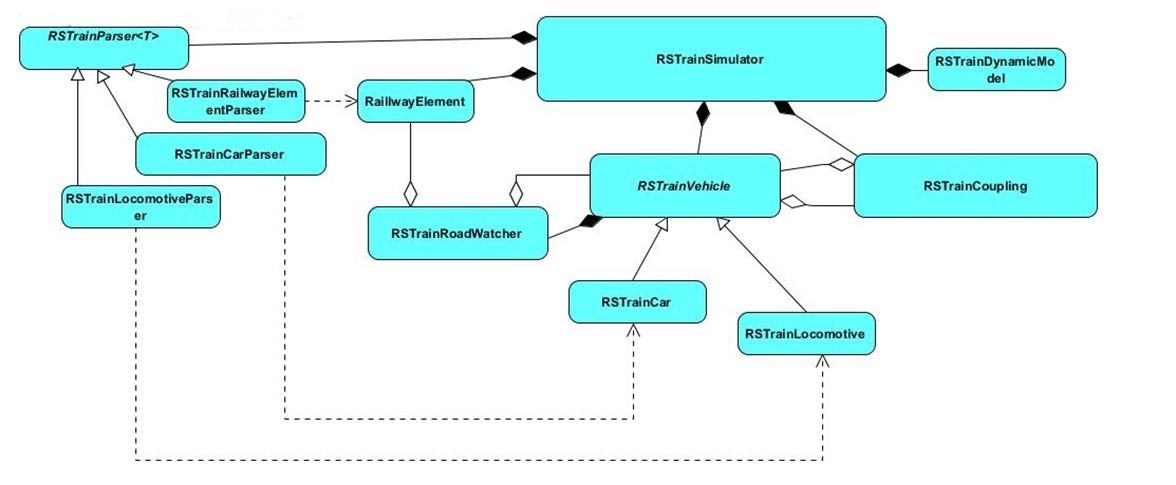
\includegraphics[scale=0.5]{resimler/uml.jpg} 
\end{figure}

Elde edilen tasarım sonucunda, proje çıktısı sonucunda beklenen çıktıların karşılanması mümkün kılınmış ve sisteme ekleme yapılması sonucunda ortaya çıkacak değişiklikler minimize edilmiştir. Tasarım sürecinde , factory, strategy, singleton, observer patternlerine başvurulmuştur.

\subsection{Sınıfların Oluşturulması ve İlgili Fonksiyonların Yazılması}
yapıyı kur sınıfları ve fonksıyonları guzel ıfade etmek gerek
\begin{itemize}
\item RSTrainParser: Sistemin kullanacağı XML dosyalarını işleyen sınıfların temel sınıfıdır. Kendisinden türetilen sınıflar, bu sınıfın barındırdığı sanal fonksiyonu gerçeklemek zorundadırlar. 
\item RSTrainLocomotiveParser :
\end{itemize}

\subsection{XML Yapısı}

\newpage

\section{Testler}
Sistemin doğru çalıştığını göstermek hataları gidermek için belli testler yapılacaktır. Sistemin doğruluğu sağlandıktan sonra performans testleri gerçekleştirilecektir. Her test aşamasında ne ölçüleceği, nasıl ölçüleceği ve tahmini sonuçlar verilmiştir. Ardından yapılan testler için sonuçlar sunulmuştur. Testler ana bölümlere ayrılmış, bu ana bölümlerde alt testler olarak parçalanmışlardır.

\subsection{Motor Testleri}
Lokomotifin motor değerleri ,tahrik kuvveti ile ilgili değerler incelenecektir. Ayrıca motorlar tarafından harcanan güç değeri, ve voltaj akım değerleri testleri yapılacaktır.

\subsubsection{Tahrik Kuvveti}
\begin{itemize}
\item \textbf{Test:} Motor tarafından sağlanan tahrik kuvvetinin grafik üzerinden okunan değerler ile eş olması.\\
\item \textbf{İncelecek Değişken:} ThrottleForce değişkeni incelenecektir.\\
\item \textbf{Beklenti:} Motor grafiği üzerindeki değerler ile tutması.\\
\item \textbf{Test Koşulları:} Bu test için sadece bir lokomotif yaratılıacak ve farklı motor kolu konumlarında değişkenler incelenecek.\\
\item \textbf{Sonuç:}
\end{itemize}

\subsubsection{Akım ve Güç Değerleri}
\begin{itemize}
\item \textbf{Test:} Motor tarafından sağlanan kuvvet ve hız değerlerinin akım ve voltaj değerleri ile hesaplanan güç değerleriyle uygun olması. Verimlilik konusunda çalışılması gerekli\\
\item \textbf{İncelecek Değişken:} ThrottleForce, velocity, akım ve voltage değişkeni incelenecektir.\\
\item \textbf{Beklenti:} Güç değerlerinin yaklaşık çıkması\\
\item \textbf{Test Koşulları:} Bu test için sadece bir lokomotif yaratılıacak ve farklı motor kolu konumlarında değişkenler incelenecek.\\
\item \textbf{Sonuç:}
\end{itemize}

\subsubsection{Dinamik Fren}
\begin{itemize}
\item \textbf{Test:} Motor tarafından uygulanana dinamik fren kuvvetlerinin grafik ile eşleşmesi.\\
\item \textbf{İncelecek Değişken:} dynamicBrakeForce değişkeni incelenecek.\\
\item \textbf{Beklenti:} Değerlerin grafik ile eşleşmesi.\\
\item \textbf{Test Koşulları:} Bu test için sadece bir lokomotif yaratılıacak ve farklı dinamik fren kolu konumlarında değişkenler incelenecek.\\
\item \textbf{Sonuç:}
\end{itemize}

\subsubsection{Patinaj}
\begin{itemize}
\item \textbf{Test:} Tekerlek üzerine etki eden motor ve fren kuvvetlerinin toplamının patinaj değeriyle karşılaştırılması.\\
\item \textbf{İncelecek Değişken:} Aderans kuvveti, motor kuvveti, fren kuvvetleri\\
\item \textbf{Beklenti:} Aderans deperinin verilen grafikledeki gibi olması, belirli konumlarda (ör:dururken yüksek kademelerde motor kuvveti) aracın kayması.\\
\item \textbf{Test Koşulları:} Bu test için sadece bir lokomotif yaratılıacak ve farklı tahrik ve fren konumlarında kayma durumları incelenecek. Ayrıca hız ile aderans kuvvetinin değişimi incelenecek.\\
\item \textbf{Sonuç:}
\end{itemize}

\subsection{Hava Freni}
Hava freni ile ilgili olan testler. Öncelikle lokomotifin kondüvit hattındaki değişimleri etkileyen makinist musluğu ve modrabl musluğunun çalışma şekilleri incelenecektir. Sonra kondüvit hattında basınç değerlerinin ilerlemesi ve hataların basınç üzerindeki etkileri incelenecek. Daha sonra kontrol valfının çalışma prensipleri ve fren değerleri üzerindeki etkileri incelenecek. Fren değerlerinin doğruluğu ve motor ve fren değerleri ile karşılaştırılması yapılacaktır.

\subsubsection{Makinis Musluğu Çalışma Şekli}
zamanları girmen ve detayları girmen gerek
\begin{itemize}
\item \textbf{Test:} 
\begin{enumerate}
\item Makinis musluğu 1. konumda iken 5 saniye içinde basınç sıfıra düşecek
\item Makinis musluğu 2. konumda iken basınç değerinin zamana bağlu olarak azalması
\item Makinis musluğu 3. konumda iken basınçlar değişmeyecek
\item Makinis musluğu 4. konumda iken basınç değerinin zamana bağlı olarak artması
\item Makinis musluğu 5. konumda iken 5 saniye içinde basınç 7atm ye çıkacak
\end{enumerate}
\item \textbf{İncelecek Değişken:} Makinis musluğu konumu, ilk araç üzerindeki kondüvit basıncı değişimi.\\
\item \textbf{Test Koşulları:} Bu test için sadece bir lokomotif yaratılacak ve makinist musluğunun konumu değiştirilerek basınç incelenecek.\\

\item \textbf{Beklenti:} Kondüvit basıncının istenilen şekilde değişmesi bekleniyor.\\
\item \textbf{Sonuç:}
\end{itemize}

\subsubsection{Modrabl Musluğu}
zamanları girmen ve detayları girmen gerek
\begin{itemize}
\item \textbf{Test:} 
\begin{enumerate}
\item Makinis musluğu 1. konumda iken basınç değerini yaşav azaltacak
\item Makinis musluğu 2. konumda iken basınç değeri değişmeyecek
\item Makinis musluğu 3. konumda iken basınç değeri yavaş artacak
\item Makinis musluğu 4. konumda iken basınç 5 saniye içinde doldur
\end{enumerate}
\item \textbf{İncelecek Değişken:} Makinis musluğu konumu, kontüvit basıncı ilk değeri.\\
\item \textbf{Beklenti:} İstenilen değerlerde değişmesi gerekmektedir. Ayrıca makinist musluğu ile beraber çalışması incelenecektir.\\
\item \textbf{Test Koşulları:} Bu test için sadece bir lokomotif gerekmektedir. \\
\item \textbf{Sonuç:}
\end{itemize}

\subsubsection{Purjör Butonu}
\begin{itemize}
\item \textbf{Test:} Purjör botonun çalışması test edilecektir.\\
\item \textbf{İncelecek Değişken:} Kondüvit basınç değeri\\
\item \textbf{Beklenti:} .Purjör basıldığında kondüvit hattı üzerinde makinist musluğu lokomotif devredışı kalmalı ve modrabl musluğu ile yönetilmeli.\\
\item \textbf{Test Koşulları:} Bu test için sadece bir lokomotif gerekmektedir. \\
\item \textbf{Sonuç:}
\end{itemize}

\subsubsection{Kondüvit hattı basınç ilerlemesi}
\begin{itemize}
\item \textbf{Test:} Kondüvit hattı üzerinde basınç değerlerinin ilerleme hızı ve şeklinin takip edilmesi\\
\item \textbf{İncelecek Değişken:} Kondüvit basınç değeri\\
\item \textbf{Beklenti:} .Basınç değerleri makinist musluğu ile kontrol edilirken vagonlara uygun hızda ve şekilde aktarılmalı.\\
\item \textbf{Test Koşulları:} Bu test için lokomotif ve vagon hattı gerekmektedir. \\
\item \textbf{Sonuç:}
\end{itemize}

\subsubsection{Kondüvit hattı hataları}
\begin{itemize}
\item \textbf{Test:} Kondüvit hattı üzerinde oluşan hataların basınç akışı üzerinde etkisi incelenecektir\\
\item \textbf{İncelecek Değişken:} Kondüvit basınç değeri\\
\item \textbf{Beklenti:} Tıkanma, kaçak olma, kopme durumlarında kondüvit üzerinde basınç akışı.\\
\item \textbf{Test Koşulları:} Bu test için lokomotif ve vagon hattı gerekmektedir. \\
\item \textbf{Sonuç:}
\end{itemize}


\subsubsection{Kontrol Valfı Çalışma Testleri}
\begin{itemize}
\item \textbf{Test:} .Kondüvit hattı üzerinde basınç değerlerine göre yedek depo basınçlarının ve fren silindiri basınçlarının incelenmesi\\
\item \textbf{İncelecek Değişken:} Yedek hava deposu basıncı ve fren silindiri basıncı\\
\item \textbf{Beklenti:} Kontrol valfının çalışma prensibine göre tepki vermelidir.\\
\item \textbf{Test Koşulları:} Bu test için bir lokomotif yeterlidir.\\
\item \textbf{Sonuç:}
\end{itemize}


\subsubsection{Kontrol Valfı Hataları}
\begin{itemize}
\item \textbf{Test:} Kontrol valfı üzerinde oluşan hataların takip edilmesi\\
\item \textbf{İncelecek Değişken:} Yedek hava deposu basıncı ve fren silindiri basıncı\\
\item \textbf{Beklenti:} Hatalara uygun tepki vermesi\\
\item \textbf{Test Koşulları:} Bu test için bir lokomotif gerekmektedir.\\
\item \textbf{Sonuç:}
\end{itemize}


\subsubsection{Fren Değerleri}
\begin{itemize}
\item \textbf{Test:} Fren silindirinde oluşan basınca göre oluşan fren değerlerinin incelenmesi\\
\item \textbf{İncelecek Değişken:} Fren değeri\\
\item \textbf{Beklenti:} Uygun fren değerlerinin oluşması\\
\item \textbf{Test Koşulları:} Bu test için bir lokomotif gereklidir. \\
\item \textbf{Sonuç:}
\end{itemize}

\subsection{Araçlar Arası Kuvvetler}
\begin{itemize}
\item \textbf{Test:} Araçlar arası uzaklıklara bağlı olarak oluşan kuvvetler incelenecektir\\
\item \textbf{İncelecek Değişken:} Araçlar arası kuvvet değerleri\\
\item \textbf{Beklenti:} Araçlar arasındaki kuvvet değerlerinin uzaklık ile değişiminin grafikteki gibi olması\\
\item \textbf{Test Koşulları:} Bu test için lokomotif ve vagon gerekmektedir. \\
\item \textbf{Sonuç:}
\end{itemize}

\subsection{Yol Değerleri}
\begin{itemize}
\item \textbf{Test:} Yolun belli konumlarındayken yol özelliklerinin doğru olması\\
\item \textbf{İncelecek Değişken:} Yol değerleri, rampa eğimi, dönüş yarıçapı\\
\item \textbf{Beklenti:}  Değerlerin iroad dosyasındakiler ile aynı olması\\
\item \textbf{Test Koşulları:} Bu test için bir lokomotif gerekmektedir. \\
\item \textbf{Sonuç:}
\end{itemize}

\subsubsection{Section ve Kısımların Doğru Hesaplanması}
\begin{itemize}
\item \textbf{Test:} Yolun belli konumlarındayken yol tanımlarının doğru hesaplanması\\
\item \textbf{İncelecek Değişken:} Section ve kısım değerleri\\
\item \textbf{Beklenti:} Yol konumu bilinirken section ve kısım değerlerinin iRoad dosyasındakilerle aynı olması\\
\item \textbf{Test Koşulları:} Bu test için bir lokomotif gerekmektedir. \\
\item \textbf{Sonuç:}
\end{itemize}


\subsubsection{Trenin Yön Ayarlarının Dorğu Olması}
\begin{itemize}
\item \textbf{Test:} Trenin pozitif yönünün doğru olması ve kuvvetlerin ona göre doğru hesaplanması\\
\item \textbf{İncelecek Değişken:} Kuvvet ve hız değerlerinin yönü\\
\item \textbf{Beklenti:} Kuvvet ve hızın yöne göre uygun şekilde olmas\\
\item \textbf{Test Koşulları:} Bu test için bir lokomotif gerekmektedir. \\
\item \textbf{Sonuç:}
\end{itemize}


\subsection{Fren Süresi}
\begin{itemize}
\item \textbf{Test:} Belirlenmiş bir yolda trenin belli bir hızda fren yapma süresi ölçülecektir\\
\item \textbf{İncelecek Değişken:} Durma süresi\\
\item \textbf{Beklent:} DUrma süresinin gerçek tren ile benzer olması\\
\item \textbf{Test Koşulları:} Bu test için gerçek değerlerdeki konfigurasyonun sağlanması gerekmektedir \\
\item \textbf{Sonuç:}
\end{itemize}

\subsection{Sefer Değerleri Karşılaştırılması}
\begin{itemize}
\item \textbf{Test:} Kayıt edilen gerçek bir sefer esnasındaki değerlerin simulatör ile karşılaştırılması\\
\item \textbf{İncelecek Değişken:} Gerçek tren üzerinde okunan bütün değerler \\
\item \textbf{Beklenti:} Okunan değerlerin gerçek değerler ile yakın olması\\
\item \textbf{Test Koşulları:} Bu test için gerçek testeki konfigurasyonun aynısının oluşturulması gerekmektedir. \\
\item \textbf{Sonuç:}
\end{itemize}

\subsection{Performans Testleri}

\subsubsection{Maximum Vagon Sayısı}
\begin{itemize}
\item \textbf{Test:} 50ms yi geçirmeden maximum hesaplanabilen vagon sayısı\\
\item \textbf{İncelecek Değişken:} Vagon sayısı\\
\item \textbf{Sonuç:}
\end{itemize}

\subsubsection{Hesaplama Hızı}
\begin{itemize}
\item \textbf{Test:} Normal bir katarın hesaplama süresi ile gerçek zaman arasındaki oran\\
\item \textbf{İncelecek Değişken:} Hesaplama hızı\\
\item \textbf{Sonuç:}
\end{itemize}

\newpage
\section{Yapılacaklar}
\begin{itemize}
\item Ranfor acuple eklenecek
\item Akım ve güç modelleri eklenecek
\item Switchlerin road\_watcher da çalışması hazırlanacak
\item testler belirlenecek
\item makinist musluğu alt ve üst basınç korumaları eklenecek
\item fren silindiri basıncında problem var (artış değeri yanlış)
\item kumlama ve patinaj eklenecek
\item Slope degerinin birimini ogren
\item Vehicle icinde kutle degeri incelenecek bigimi N mu yoksa kg mi?
\item Vehocle altinda adheranceforce da kutlu degerine uygun degisikligi yap? xxxpa
\item Vehicle altinda coefficient of frictioni incele
\item Vehicle altinda calcControlValve ve calcBrakeForce fonksiyonlarini kaldir
\item Locomotive altinda auxbrake degerine gerek yok
\item Yon konusunu netlestir
\end{itemize}


\newpage
\section{Ekler}

\end{document}
